\documentclass[
    12pt,
    a4paper,
    addpoints,
    answers,
    convocatoria=ord,
    titulacion=NoCD,
    curso=2023/2024,
]{db-exam}

\begin{document}

\begin{questions}

\question[2\half] \textbf{Modelado.}

Una compañía de seguros médicos tiene una base de datos en la que almacena su información referente a sus instalaciones, médicos, tipos de pruebas que puede realizar y qué técnicos pueden participar en la realización de esos tipos de pruebas. Con esta base de datos, están gestionando de forma manual la asistencia a consultas y pruebas de los pacientes, pero necesitan automatizar esta parte de la gestión. Somos contratados para atender esta necesidad. Para empezar, al realizar la ingeniería inversa de la Base de Datos existente (¡Qué suerte, implementada en MySQL Workbench!), obtenemos el siguiente diagrama que resume la estructura de la base de datos:

\begin{center}
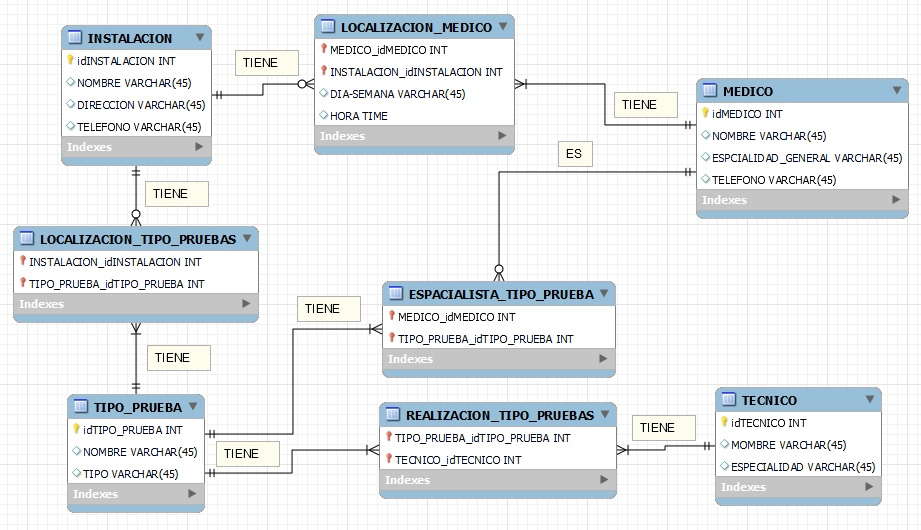
\includegraphics[width=0.9\textwidth]{figs/bbdd-2023-2024-ordinaria/mer-enunciado.jpg}
\end{center}

A partir de ahora y añadiendo elementos a esta base de datos debemos atender lo siguiente: 

Se darán de alta los pacientes existentes (actualmente en un fichero externo), dando el número de asegurado, que será único, nombre, fecha de nacimiento, dirección, teléfono y correo electrónico. 

Existirá una APP que permita a los pacientes consultar qué médicos hay existen por especialidad en las distintas instalaciones y pedir una consulta con ellos. En la consulta se indicará en qué instalación se va a realizar, qué médico la va a atender y, por supuesto, para qué paciente. También se indicará la fecha y la hora de la consulta. El sistema enviará al teléfono del paciente un SMS 24 horas antes de cada consulta un mensaje de recordatorio. El paciente podrá anular su consulta en ese o en cualquier otro momento. Después de pasar consulta, el médico puede escribir un informe al respecto que será un texto sin limitación de espacio y también puede solicitar que se realicen una serie de tipos de pruebas referentes a la consulta.

Cuando se solicita una prueba de un tipo en particular, se debe registrar una descripción de la prueba a realizar, la fecha y la hora de la prueba, la instalación en la que se va a realizar y para qué paciente. La prueba también podrá contener un campo de texto sin límite en el que se escriba un informe de resultados por parte de un médico (si es una prueba en la que participa un médico). También se tiene que registrar qué técnico o técnicos pueden haber estado asignados a la prueba. 

Por último, será necesario tener almacenado el número de consultas pedidas por cada paciente a través de esta nueva funcionalidad y así tener una idea del gasto por cada paciente.

Se pide: 

\begin{itemize}
    \item Realizar un Modelo Entidad-Relación utilizando notación Chen que incluya el diagrama que representaría el esquema de base de datos obtenido por MySQL Workbemch e incorpore tantas modificaciones que consideren necesarias para satisfacer los nuevos requisitos.
    \item Justificar al menos cuatro cardinales mínimas del modelo propuesto.
\end{itemize}

\begin{solution}
    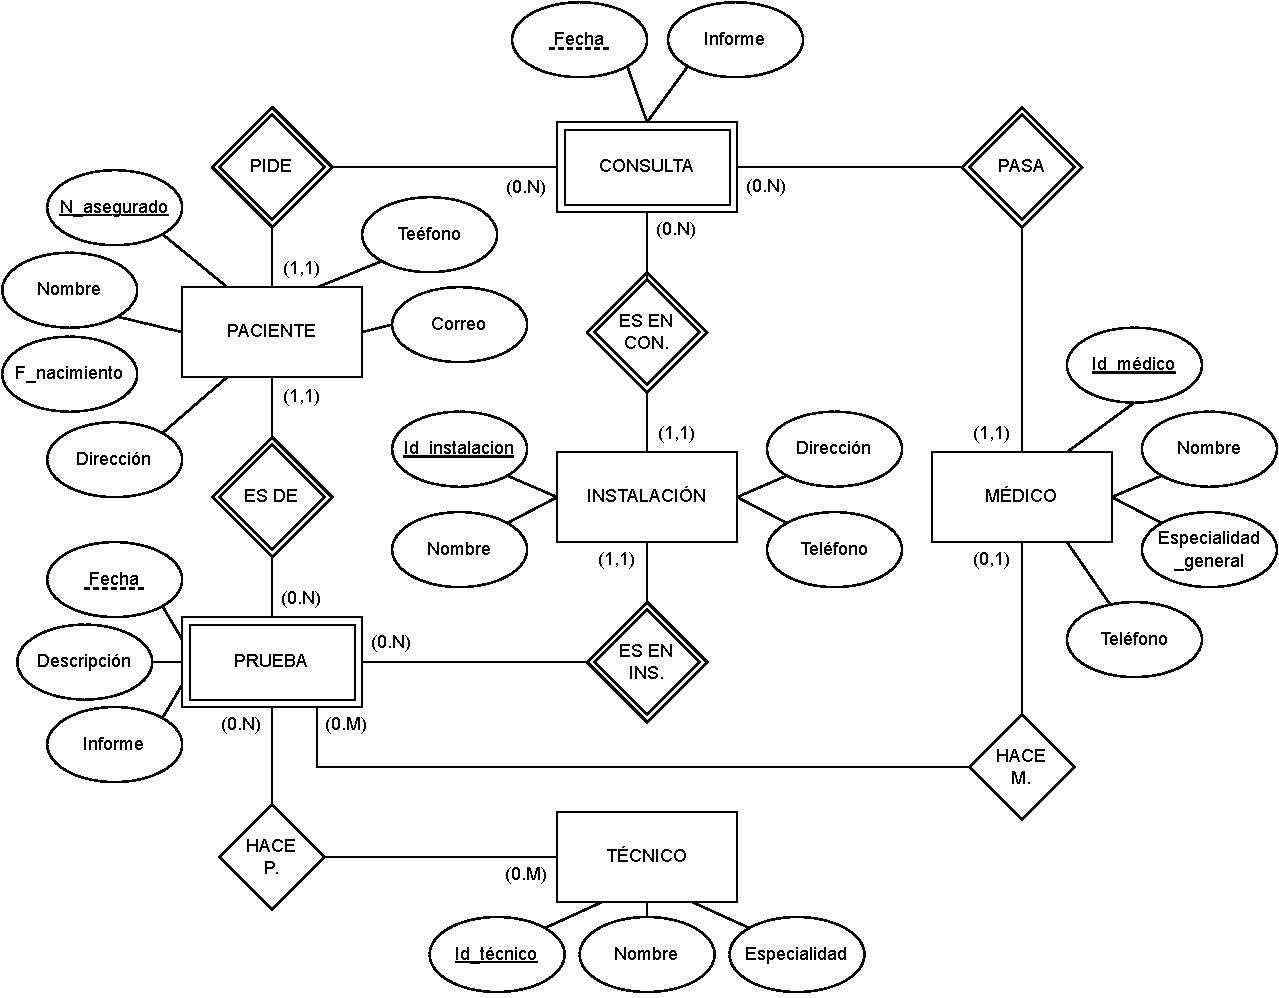
\includegraphics[width=\textwidth]{figs/bbdd-2023-2024-ordinaria/mer-solucion.pdf}

    Justificación de cardinalidades mínimas:
    \begin{itemize}
        \item Del texto ``\textit{También se tiene que registrar qué técnico o técnicos pueden haber estado asignados a la prueba. }'' se infiere que los técnicos pueden o no realizar una prueba, por eso \texttt{HACE P.} es 0 en el lado de \texttt{PRUEBA}.
        \item Del texto ``\textit{En la consulta se indicará [...] para qué paciente}'' se define que la cardinalidad mínima de \texttt{PIDE} es 1 en el lado de \texttt{PACIENTE}.
        \item Del texto ``\textit{En la consulta se indicará [...] qué médico la va a atender}'' se extrae que la consulta debe ser atendida por un médico, por lo que la cardinalidad mínima de \texttt{PASA} en el lado de \texttt{MÉDICO} es 1.
        \item Del texto ``\textit{Cuando se solicita una prueba de un tipo en particular, se debe registrar [...] para qué paciente}'' se restringe que la cardinalidad mínima de \texttt{ES DE} es 1 en el lado de \texttt{PACIENTE}.
    \end{itemize}
\end{solution}

\newpage
\question[1\half] \textbf{Álgebra relacional.}

Un recién titulado en el Grado de Informática por nuestra escuela, ha puesto su empeño en mejorar el rendimiento del tradicional juego Pokemon y optimizar el uso que hace de los recursos móviles. Para ello ha propuesto una mejora de la Base de Datos basada en el siguiente Modelo Entidad-Relación:

\begin{center}
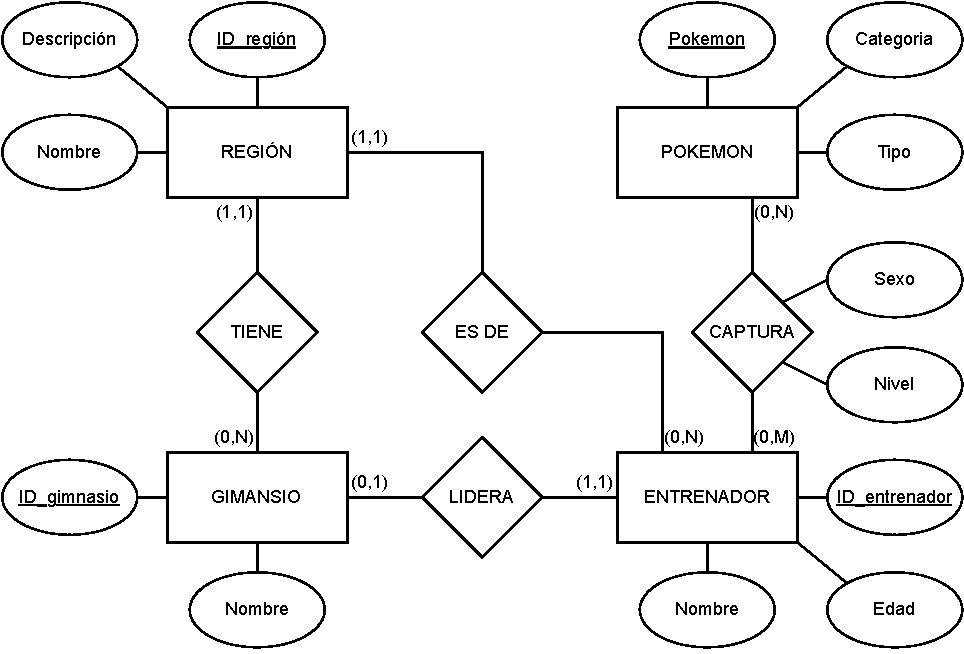
\includegraphics[width=0.8\textwidth]{figs/bbdd-2023-2024-ordinaria/mer-pokemon.pdf}
\end{center}

Tras un proceso de paso a tablas, ha obtenido el siguiente modelo relacional:

\begin{center}
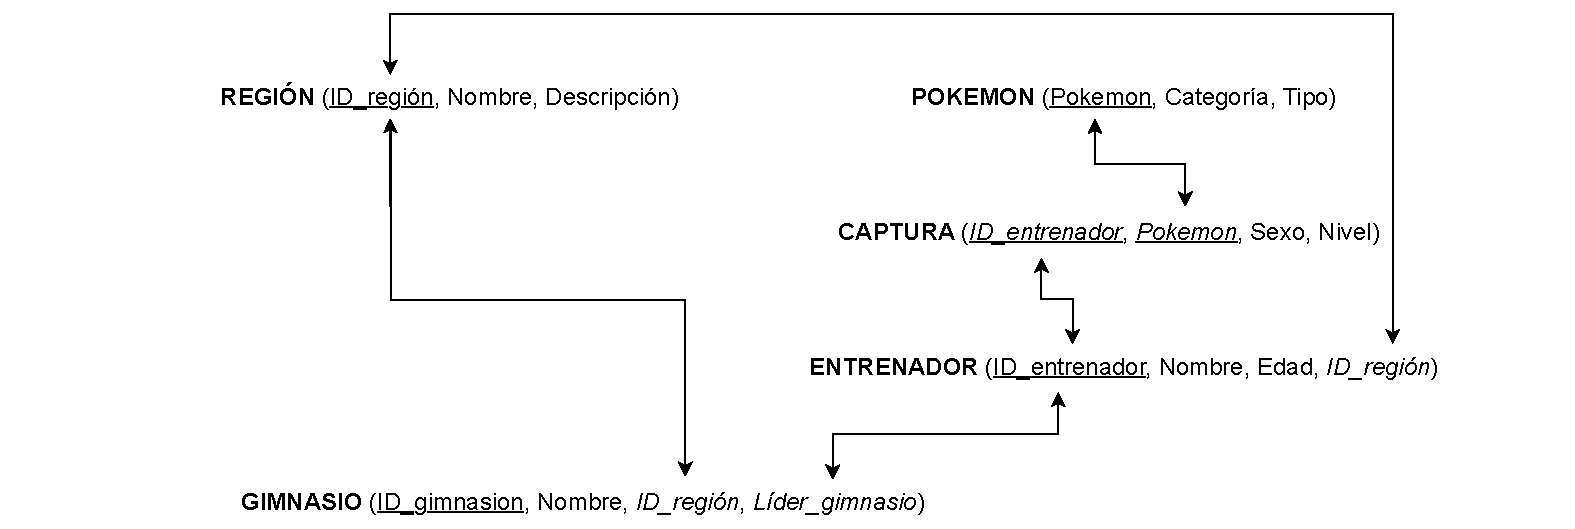
\includegraphics[width=\linewidth]{figs/bbdd-2023-2024-ordinaria/relacional-pokemon.pdf}
\end{center}

\newpage

Ahora quiere evaluar el rendimiento de sus sistema por lo que se ha planteado resolver las siguientes consultas empleando álgebra relacional y SQL.

\newpage  
\begin{parts}
\part[\half] Obtener los pokemon y su categoría de aquellos cuyo entrenador sea originario de la región con identificador \texttt{30}.
\begin{solution}
$\Pi_{Pokemon, Categoria}(POKEMON \bowtie$

$\sigma_{ID\_region=30}(ENTRENADOR \bowtie CAPTURA))$
\end{solution}
    
\part[\half] Obtener el nombre de las regiones de las que proceden los entrenadores que solo tienen pokemons tipo ``\textit{Planta}''.
\begin{solution}   
$\Pi_{Nombre}(REGION\bowtie \Pi_{ ID\_entrenador,ID\_region }(ENTRENADOR) \bowtie$

$(\Pi_{ ID\_entrenador}( \sigma_{Tipo="Planta"} (CAPTURA  \bowtie POKEMON))$

$-$

$\Pi_{ ID\_entrenador}( \sigma_{Tipo<>"Planta"} (CAPTURA  \bowtie POKEMON)) )$
\end{solution}

\part[\half] Obtener los identificadores de los entrenadores que han logrado capturar todos los pokemon.
\begin{solution}   
$\Pi_{ID\_entrenador, Pokemon}(CAPTURA)$

$\%$

$\Pi_{Pokemon}(POKEMON)$
\end{solution}
\end{parts}

\newpage
\question[2] \textbf{SQL.}

Empleando el modelo relacional del ejercicio 2, resuelva las siguientes consultas en lenguaje SQL.
  
\begin{parts}

\part[\half] Obtener el nombre de los entrenadores que no han capturado ningún pokemon de tipo fuego. 

\begin{solution}
\begin{lstlisting}[language=SQL]
SELECT nombre
FROM entrenador
WHERE id_entrenador NOT IN 
       (SELECT id_entrenador
        FROM captura
          INNER JOIN pokemon ON captura.pokemon = pokemon.pokemon
        WHERE tipo = 'Fuego');
\end{lstlisting}
\end{solution}

\part[\half] Obtener el nombre de los pokemon que han sido capturados por todos los entrenadores de la región de `\textit{Kanto}'.

\begin{solution}
\begin{lstlisting}[language=SQL]
SELECT pokemon
FROM captura
  INNER JOIN entrenador 
    ON entrenador.id_entrenador = captura.id_entrenador
  INNER JOIN region 
    ON region.id_region = entrenador.id_region
WHERE region.nombre = 'Kanto'
GROUP BY pokemon
HAVING COUNT(DISTINCT id_entrenador) = 
         (SELECT COUNT(*)
          FROM entrenador
            INNER JOIN region 
              ON region.id_region = entrenador.id_region
          WHERE region.nombre = 'Kanto');
\end{lstlisting}
\end{solution}

\newpage

\part[\half] Obtener el nombre de los entrenadores que han capturado a `\textit{Mew}' y `\textit{Mewtwo}'. 

\begin{solution}
\begin{lstlisting}[language=SQL]
SELECT nombre
FROM entrenador
WHERE id_entreandor IN (SELECT id_entreandor
                        FROM captura
                        WHERE pokemon = 'Mew')
  AND id_entrenador IN (SELECT id_entreandor
                        FROM captura
                        WHERE pokemon = 'Mewtwo');
\end{lstlisting}
\end{solution}

\part[\half] Incrementar en 1 el nivel de todos los pokemons del entrenador que haya capturado al pokemon con el nivel más bajo. 

\begin{solution}
\begin{lstlisting}[language=SQL]
UPDATE captura
SET nivel = nivel + 1
WHERE id_entreandor IN (SELECT id_entrenador
                        FROM captura
                        WHERE nivel <= ALL (SELECT nivel
                                            FROM captura));
\end{lstlisting}
\end{solution}

\end{parts}

\newpage
\question[1\half] \textbf{Procedimientos, funciones y triggers.}

Basándonos en la base de datos resultante del modelo relacional propuesto en el ejercicio 2, escribir la sentencia SQL para añadir una nueva columna en la tabla \texttt{REGIÓN} que se llame \texttt{Lider\_región} incluyendo la parte de integridad referencial que debería ir asociada a dicha columna. A continuación escribir un \emph{PROCEDIMIENTO} que calcule por cada región cual es el entrenador, entre todos los que pertenezcan a la región, que ha realizado el mayor número de capturas de pokemons con nivel máximo del global de la base de datos, y que actualice la tabla \texttt{REGIÓN} poniendo dicho entrenador como lider de la región correspondiente. Será obligatorio el uso de un \texttt{CURSOR} para implementar este procedimiento. En caso de que varios entrenadores cumplan la condición, se deberá escoger únicamente uno de ellos arbitrariamente (utilizar \texttt{LIMIT 1} para restringir el número de resultados a 1).
        
\begin{solution}
\begin{lstlisting}[language=SQL]
ALTER TABLE region ADD COLUMN lider_region INTEGER NULL;
ALTER TABLE region ADD CONSTRAINT fk_region_entrenador
FOREIGN KEY (lider_region) REFERENCES entrenador(id_entrenador);

DELIMITER $$
CREATE PROCEDURE actualizarLiderRegion ()
BEGIN
    DECLARE id_lider, id_reg INTEGER;
    DECLARE done INT DEFAULT FALSE;
    DECLARE cur1 CURSOR FOR SELECT id_region FROM region;
    DECLARE CONTINUE HANDLER FOR NOT FOUND SET done = TRUE;
    
    OPEN cur1;
    read_loop: LOOP
        FETCH cur1 INTO id_reg;
        IF done THEN
            LEAVE read_loop;
        END IF;
        
        SELECT id_entrenador INTO id_lider
        FROM captura NATURAL JOIN entrenador 
        WHERE entreandor.id_region = id_reg 
          AND captura.nivel = (SELECT MAX(nivel) 
                               FROM captura)
        GROUP BY captura.id_entrenador
        HAVING COUNT(*) >= 
            (SELECT COUNT(*) 
             FROM captura NATURAL JOIN entrenador 
             WHERE entrenador.id_region = id_reg 
               AND captura.nivel = (SELECT MAX(nivel) 
                                    FROM captura)
             GROUP BY captura.id_entrenador)
        LIMIT 1;
        
        UPDATE region
        SET region.lider_region = id_lider
        WHERE id_region = id_reg
    END LOOP;
    CLOSE cur1;
    
END$$
DELIMITER ;
\end{lstlisting}
\end{solution}

\newpage
\question[\half] \textbf{Formas normales.}

¿Qué pasos deberían darse para que la base de datos siguiente cumpliera la primera forma normal (1FN)?
    
\vspace{1em}

\begin{tabular}{lllll}
\hline
ID & Nombre & Edad & Ciudad & Pokemon \\
\hline
1 & Ash & 15 & Pueblo Paleta & Pikachu, Bulbasaur, Charmander \\
2 & Misty & 13 & Ciudad Celeste & Psyduck, Starmie \\
3 & Brock & 16 & Ciudad Plateada & Onix, Geodude, Zubat \\
\hline
\end{tabular}  

\begin{solution}
Actualmente existe más de un valor para el atributo \texttt{Pokemon}, por lo que se debería crear una nueva tabla que guardase \texttt{ID}, \texttt{Pokemon} para evitar que esto sucediera. En la tabla actual habría que eliminar la columna \texttt{Pokemon}.
\end{solution}

\newpage
\question[1] \textbf{Programación.}

El siguiente modelo entidad-relación pertenece a una base de datos de una gestora de comercios farmacéuticos.

\begin{center}
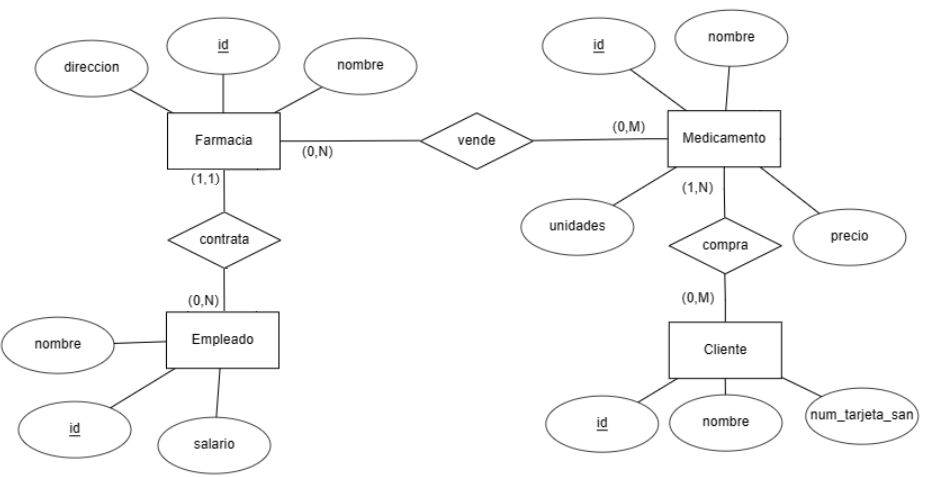
\includegraphics[width=0.8\textwidth]{figs/bbdd-2023-2024-ordinaria/mer-programacion.png}
\end{center}

En dicha base de datos se quiere llevar un control de los empleados que trabajan en cada farmacia, los medicamentos que dispone, así como los medicamentos que adquieren los clientes mediante su tarjeta sanitaria.

Realice el etiquetado de clases y sus atributos para que mediante el ORM \textbf{Hibernate} de Java pueda realizar la conexión con la base de datos satisfactoriamente cumpliendo con el modelo relacional mostrado anteriormente.
  
\begin{verbatim}

            
public class Farmacia {
    

    private Long id;


    private String nombre;

    
    private String direccion;


    private Set<Medicamento> medicamento;


    private Set<Empleados> empleados;

    /*Constructor de la clase, getters, setters,...*/
}


public class Empleados {
    

    private Long id;

 
    private String nombre;
    
    private float salario;


    
    private Farmacia farmacia;
    
    /*Constructor de la clase, getters, setters,...*/
}


public class Medicamento {
    

    private Long id;

  
    private String nombre;


    private float precio;


    private int unidades;

    
    private Set<Farmacia> farmacias;

    
    private Set<Cliente> clientes;
 
    /*Constructor de la clase, getters, setters,...*/
}


public class Cliente {
    

    private Long id;

    
    private String nombre;

    
    private String num_tarjeta_san;


    private Set<Medicamento> medicamentos;
    
    /*Constructor de la clase, getters, setters,...*/
}
\end{verbatim}
  
\begin{solution}
\begin{verbatim}
@Entity
@Table(name="Farmacia")
public class Farmacia {
    @Id
    @GeneratedValue
    @Column(name="id", unique = true, nullable = false)
    private Long id;

    @Column(name="nombre", nullable = false)
    private String nombre;

    @Column(name="direccion")
    private String direccion;

    @ManyToMany
    @JoinTable(name="vende")
    private Set<Medicamento> medicamento;

    @OneToMany(mappedBy="farmacia")
    private Set<Empleado> empleados;

     /*Constructor de la clase, getters, setters,...*/
}

@Entity
@Table(name="Empleado")
public class Empleado {
    @Id
    @GeneratedValue
    @Column(name="id", unique=true, nullable=false)
    private Long id;

    @Column(name="nombre")
    private String nombre;

    @Column(name="salario")
    private float salario;

    @ManyToOne(optional=false)
    @JoinColumn(name="farmacia")
    private Farmacia farmacia;

    /*Constructor de la clase, getters, setters,...*/
}

@Entity
@Table(name="Medicamento")
public class Medicamento {
    
    @Id
    @GeneratedValue
    @Column(name="id", unique=true, nullable=false)
    private Long id;

    @Column(name="nombre")
    private String nombre;

    @Column(name="nombre")
    private float precio;

    @Column(name="unidades")
    private int unidades;

    @ManyToMany(mappedBy="medicamento")
    private Set<Farmacia> farmacias;

    @ManyToMany(mappedBy="medicamentos")
    private Set<Cliente> clientes;
    
    /*Constructor de la clase, getters, setters,...*/
}

@Entity
@Table(name = "Cliente")
public class Cliente {
    
    @Id
    @GeneratedValue
    @Column(name="id", unique=true, nullable=false)
    private Long id;

    @Column(name="nombre")
    private String nombre;

    @Column(name="num_tarjeta_san")
    private String num_tarjeta_san;

    @ManyToMany
    @JoinTable(name="compra")
    private Set<Medicamento> medicamentos;
    
    /*Constructor de la clase, getters, setters,...*/
}
\end{verbatim}
\end{solution}

\newpage
\question[1] \textbf{Ficheros.}

Tomando como referencia el siguiente archivo \texttt{XML}, guarde TODA la información en un fichero JSON \textbf{embedido válido}.

\begin{verbatim}
<pokemons>
    <pokemon>
        <nombre>Charmander</nombre>
        <tipo>Fuego</tipo>
        <habilidad>Llamarada</habilidad>
        <altura unidad="m">0.6</altura>
        <peso unidad="kg">8.5</peso>
        <evoluciones>
            <evolucion>Charmander</evolucion>
            <evolucion>Charmeleon</evolucion>
            <evolucion>Charizard</evolucion>
        </evoluciones>
    </pokemon>
    <pokemon>
        <nombre>Squirtle</nombre>
        <tipo>Agua</tipo>
        <habilidad>Torrente</habilidad>
        <altura unidad="m">0.5</altura>
        <peso unidad="kg">9</peso>
        <evoluciones>
            <evolucion>Squirtle</evolucion>
            <evolucion>Wartortle</evolucion>
            <evolucion>Blastoise</evolucion>
        </evoluciones>
    </pokemon>
</pokemons>
\end{verbatim}
    
\begin{solution}
\begin{verbatim}
{
    "pokemons": [
        {
            "nombre": "Charmander",
            "tipo": "Fuego",
            "habilidad": "Llamarada",
            "altura": {
                "valor": 0.6,
                "unidad": "m"
            },
            "peso": {
                "valor": 8.5,
                "unidad": "kg"
            },
            "evoluciones": ["Charmander", "Charmeleon", "Charizard"]
        },
        {
            "nombre": "Squirtle",
            "tipo": "Agua",
            "habilidad": "Torrente",
            "altura": {
                "valor": 0.5,
                "unidad": "m"
            },
            "peso": {
                "valor": 9,
                "unidad": "kg"
            },
            "evoluciones": ["Squirtle", "Wartortle", "Blastoise"]
        }
    ]
}
\end{verbatim}
\end{solution}
\end{questions}
\end{document}